\chapter{2008}
\label{cha:2008}

\begin{Problema}{1}
  Jorge Luis cort� un cuadrado de papel que ten�a $20$ cms de per�metro y
  obtuvo dos rect�ngulos. Si el per�metro de uno de los rect�ngulos es
  16cm �cu�l es el per�metro del otro?
\end{Problema}

\begin{Solucion}
  Cada lado del cuadrado mide $5$ cent\'imetros. Para obtener dos rect\'angulos
hay que hacer el corte de forma paralela a uno de los lados (ver figura). Notemos que, no importando d\'onde
se haga ese corte, la suma de los per\'imetros de los rect\'angulos es siempre igual a $28$: en efecto,
los lados exteriores coinciden con los lados del cuadrado ($20$ cms), mientras que el lado interior de $4$ cms (sobre
el corte) hay que sumarlo dos veces, una por cada rect\'angulo. Concluimos que el per\'imetro del otro rect\'angulo
tiene que ser igual a $12$.
\end{Solucion}

\begin{Problema}{2}
  Un granjero descubre que si cuenta sus ovejas de dos en dos, o de
  tres en tres, o de cuatro en cuatro o de cinco en cinco, siempre le
  sobra una. Si el granjero tiene menos de cien ovejas y m�s de una,
  �cu�ntas ovejas tiene el granjero?
\end{Problema}

\begin{Solucion}
  Veamos que al contarlas de dos en dos, de tres en tres, de cuatro en
  cuatro o de cinco en cinco, siempre le sobra una, por lo tanto si
  quitamos una oveja, al contarlas nunca le sobrar\'a una, es decir,
  se puede contar en grupos de dos, tres, cuatro o cinco sin que sobre
  alguna oveja, entonces el n\'umero de ovejas debe ser un n\'umero
  que sea m\'ultiplo de dos, tres, cuatro o cinco, pero los \'unicos
  n\'umeros que son m\'uliplos de ellos son los m\'ultiplos de
  sesenta.

  Ahora como quitamos una oveja, en vez de tener m\'as de una oveja
  debe tener m\'as de cero ovejas (ya que no se considera la oveja que
  se quit\'o) y en lugar de tener menos de cien ovejas debe tener
  menos de noventa y nueve ovejas, pero el \'unico m\'ultiplo de
  sesenta entre cero y noventa y nueve es el n\'umero sesenta, por lo
  tanto el granjero tiene sesenta y un ovejas, recordando que no
  cont\'abamos a una oveja.
\end{Solucion}

\begin{Problema}{3}
  Denotemos por $f(n)$ la suma de los divisores positivos de un numero
  natural $n$. Por ejemplo, si~$n=6$ tenemos que los divisores de 6
  son 1,2,3 y 6, que sumados dan $f(6)=1+2+3+6=12$. Encuentra el valor
  de $f(n)$ m�s peque�o entre todas las $n$ mayores o iguales a 2008.
\end{Problema}

\begin{Solucion}
  
\end{Solucion}

\begin{Problema}{4}
  De una lista de~8 n�meros naturales consecutivos, se borra uno de
  los n�meros. La suma de los n�meros que quedaron despu�s de borrar
  es igual a 2008 �Cu�l es el n�mero borrado?
\end{Problema}

\begin{Solucion}
  
\end{Solucion}

\begin{Problema}{5}
  Considera el conjunto $A=\{1,2,3,\ldots,10\}$.  De cada subconjunto
  de 7 elementos de $A$ se toma el n�mero mayor �Cu�l es la suma de
  todos estos n�meros mayores?
\end{Problema}

\begin{Solucion}
  
\end{Solucion}

\begin{Problema}{6}
  Considera un cuadrado cuyo lado tiene longitud~$2$ y cuatro
  c�rculos del mismo radio con centros respectivos en los puntos
  medios del cuadrado, de tal modo que los c�rculos correspondientes a
  lados adyacentes son tangentes.  Encontrar el �rea de la regi�n
  dentro del cuadrado y fuera de los c�rculos. Es decir, en la figura
  siguiente, se pide hallar el �rea de la regi�n sombreada.

  \begin{center}
    \pgfmathsetmacro{\rad}{0.5*sqrt(2)}

    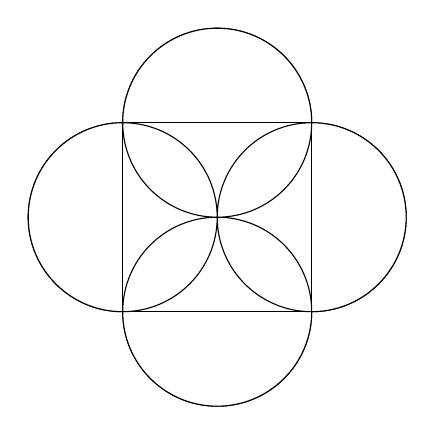
\begin{tikzpicture}[scale=1.2]
      \pgfmathparse{sqrt(2)*0.5}
      \filldraw[fill=gray,even odd rule]
      rectangle (2,2) (0,1)
      circle (\rad) (1,0)
      circle (\rad) (1,2)
      circle (\rad) (2,1)
      circle (\rad);
      \filldraw [fill=white]
      (0,1) circle (\rad)
      (1,0) circle (\rad)
      (1,2) circle (\rad)
      (2,1) circle (\rad);
      \draw rectangle (2,2);
    \end{tikzpicture}
  \end{center}
\end{Problema}


%%% Local Variables: 
%%% mode: latex
%%% TeX-master: "libro"
%%% End: 